\documentclass[xcolor=dvipsnames]{beamer}
\usepackage[english]{babel}
\usepackage[latin1]{inputenc}
\usepackage{times}
\usepackage[T1]{fontenc}
\usepackage{graphicx}
\usepackage[absolute, overlay]{textpos}
\usepackage{tikz}
\usepackage{multimedia}
\usepackage{soul}
\usepackage{cancel}
\def\urltilda{\kern -.15em\lower .7ex\hbox{\~{}}\kern .04em}
\def\deg{^{\circ}}

\setlength{\TPHorizModule}{0.01\textwidth}
\setlength{\TPVertModule}{\TPHorizModule}
\definecolor{darkyellow}{rgb}{1,0.75,0}
\definecolor{black}{rgb}{0,0,0}
\definecolor{skyblue}{rgb}{0.7,0.8,1.0}
\definecolor{black}{rgb}{0,0,0}
\definecolor{darkgrey}{rgb}{0.3,0.3,0.3}
\definecolor{medgrey}{rgb}{0.5,0.5,0.5}
\definecolor{lightgrey}{rgb}{0.8,0.8,0.8}
\definecolor{lightMahogany}{rgb}{0.9,0.8,0.8}

\newcommand{\cblue}[1]{{\color[rgb]{0.1, 0.0, 0.6} #1}}
\newcommand{\cgreen}[1]{{\color[rgb]{0.0, 0.6, 0.1} #1}}
\newcommand{\corange}[1]{{\color[rgb]{0.9, 0.5, 0.0} #1}}
\newcommand{\cbluewhen}[2]{{\color#2[rgb]{0.1, 0.0, 0.6} #1}}
\newcommand{\cgreenwhen}[2]{{\color#2[rgb]{0.0, 0.6, 0.1} #1}}
\newcommand{\corangewhen}[2]{{\color#2[rgb]{0.9, 0.5, 0.0} #1}}

\newcommand{\manual}[1]{
  \begin{tikzpicture}[x=\textwidth, y=0.82\textheight]%, >=angle 90]
    \useasboundingbox (0, 0) rectangle (1, 1);
    #1
  \end{tikzpicture}
}

%%% Custom nodes.

\newcommand{\basenode}[4]{
  \node[outer sep=6pt, anchor=#3] (#1) at (#2){#4};
}

\newcommand{\emptynode}[2]{
  \basenode{#1}{#2}{base}{}

}

\newcommand{\minipagenode}[5]{
  \basenode{#1}{#2}{#3}{
    \begin{minipage}{#4}
      \vspace*{-12pt}
      {#5}
      \vspace*{-8pt}
  \end{minipage}}

}

\newcommand{\imagenode}[5]{
  \minipagenode{#1}{#2}{#3}{#4}{%
    \includegraphics[width=\textwidth]{#5}%
  }
}

%%% Connectors.

\newcommand{\connect}[4]{%
  \draw[<->, color=darkpurple, line width=1pt, out=#3, in=#4] (#1) to (#2);
}
\newcommand{\connectcolor}[5]{%
  \draw[<->, color=#5, line width=1pt, out=#3, in=#4] (#1) to (#2);
}
\newcommand{\hconnect}[3]{%
  \draw[<->, color=darkpurple, line width=1pt]
  (#1.east) .. controls +(right:#3) and +(left:#3) .. (#2.west);
}
\newcommand{\vconnect}[3]{%
  \draw[<->, color=darkpurple, line width=1pt]
  (#1.south) .. controls +(down:#3) and +(up:#3) .. (#2.north);
}

\newenvironment{litemize}
{\usebeamercolor[fg]{item color}%
\scriptsize\begin{list}{$\bullet$}{%
\setlength{\itemindent}{0pt}%
\setlength{\labelwidth}{10pt}%
\setlength{\leftmargin}{15pt}%
}}
{\end{list}}

\mode<presentation>
{
  \usetheme{Warsaw}
  \usecolortheme[named=Mahogany]{structure}	
  \setbeamercovered{transparent}
  \setbeamercolor*{section in toc}{bg=white, fg=Mahogany}
}

%\beamerdefaultoverlayspecification{<+->}

\AtBeginSubsection[]
{
  \begin{frame}<beamer>
    \frametitle{Outline}
  \begin{columns}[t]
	\column{0.8\textwidth}
	\tableofcontents[sections={1-3}, currentsection, currentsubsection]
  \end{columns}	
  \end{frame}
}

\setbeamertemplate{subsection in head/foot shaded}
{\textcolor{structure!70!white}{\insertsubsectionhead}}
\setbeamertemplate{subsection in head/foot}{\textcolor{white}\insertsubsectionhead}

\title[{\textcolor{white} Global fits: the key to identifying new particles}]{\textcolor{white}{Global fits: the key to identifying new particles}}
\author[\textcolor{medgrey}{Pat Scott -- Mar 17 -- Uppsala}]{Pat Scott}
\institute{\small{NSERC Banting Fellow, McGill University / \\STFC Rutherford Fellow, Imperial College London}}
\date[March 17 2014]{March 17 2014}
\pgfdeclareimage[height=0.7cm]{university-logo}{McGill_crest}
\logo{\pgfuseimage{university-logo}}
\subject{Talks}

\begin{document}

\begin{frame}
  \titlepage
\end{frame}


\begin{frame}
\frametitle{Beyond the Standard Model (BSM) of Particle Physics}

\begin{columns}

\column{0.57\textwidth}
A story of complementarity\ldots

\begin{itemize}
\item \footnotesize Existing data give us some constraints
\visible<3->{\item Direct searches for dark matter constrain cross-sections with nuclei}
\visible<4->{\item Accelerator searches rule out lighter masses}
\visible<5->{\item Indirect searches for dark matter constrain annihilation cross-sections (+ some nuclear cross-sections)}
\end{itemize}

\column{0.44\textwidth}
\raggedright
\only<1-2>{\visible<2>{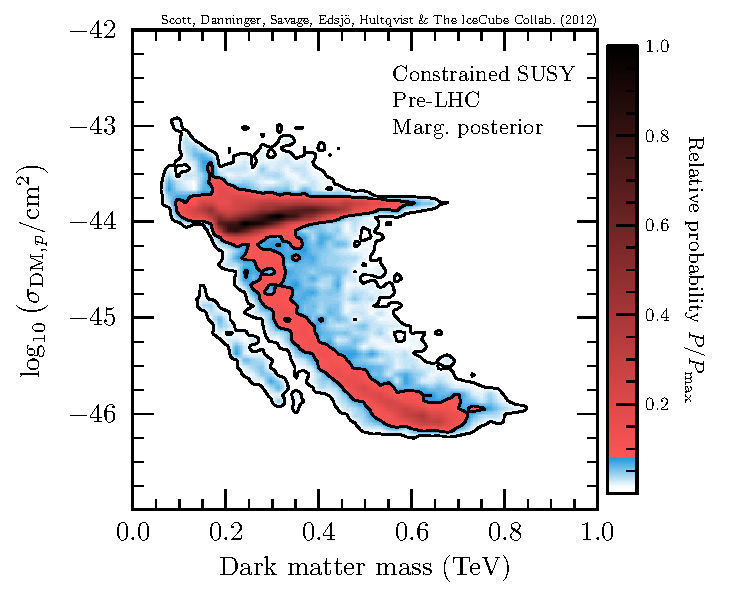
\includegraphics[height=0.95\linewidth, trim = 0 0 8 0, clip = true]{Marg2D_1_2}}}%
\only<3>{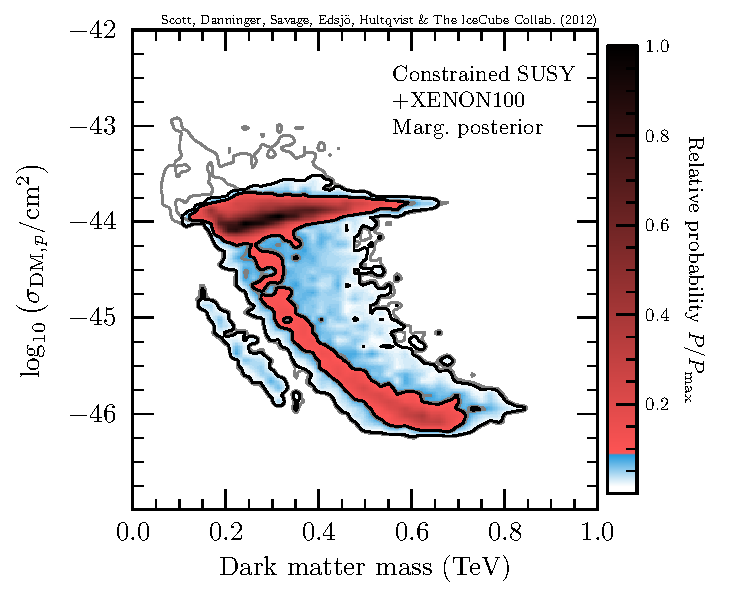
\includegraphics[height=0.95\linewidth, trim = 0 0 8 0, clip = true]{Marg2D_2_2}}%
\only<4>{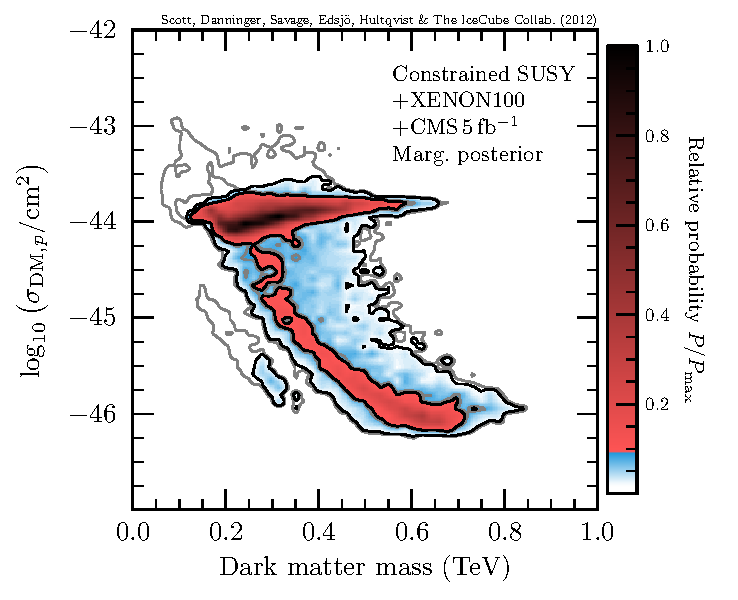
\includegraphics[height=0.95\linewidth, trim = 0 0 8 0, clip = true]{Marg2D_3_2}}%
\only<5->{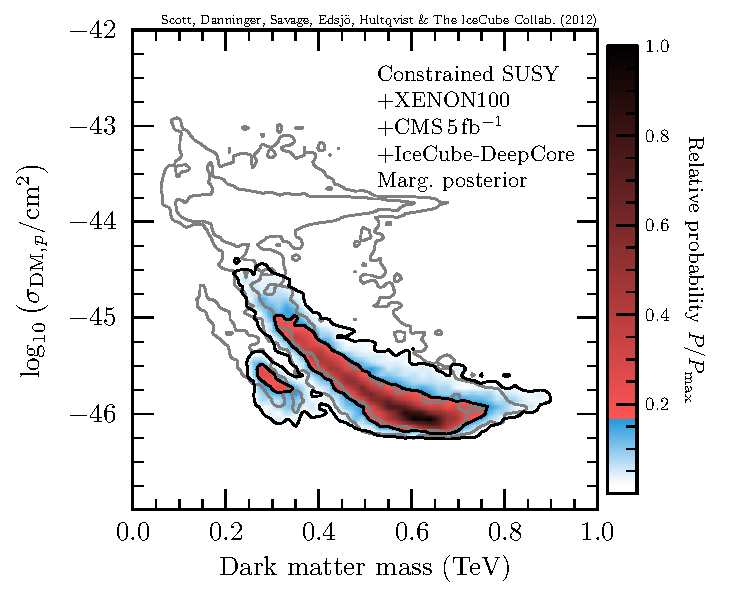
\includegraphics[height=0.95\linewidth, trim = 0 0 8 0, clip = true]{Marg2D_4_2}}

\end{columns}\vspace{5mm}

\visible<6->{\alert{My main objective} = finding/constraining new physics with astronomical AND particle data as co-navigators\vspace{3mm}}

\visible<7->{This example is a gross simplification -- the devil is in the detail.\vspace{3mm}}

\visible<7->{Many talk about complementarity, far fewer walk the walk quantitatively $\rightarrow$ global BSM fits}

\end{frame}


\begin{frame}
\frametitle{My contributions to date}

\footnotesize

\textbf{Global fits}:
\begin{enumerate}
\item Inclusion of astroparticle experiments in global fits 
\begin{itemize}
      \item first to include indirect searches for dark matter
      \item the leading producer of astroparticle global fit likelihoods
\end{itemize}
\item Improvement of statistical and numerical methods in global fits
\begin{itemize}
      \item improved optimisation/search algorithms
      \item investigated coverage properties
\end{itemize}
\end{enumerate}

\textbf{Related areas}:
\begin{enumerate}
\setcounter{enumi}{2}
\item Cutting-edge gamma-ray indirect detection constraints (first Fermi dark matter paper, best Cherenkov Telescope Array predictions) 
\item Developed \textit{ultracompact minihalos} (of dark matter) as a research field 
\item State-of-the art analysis of the scalar singlet dark matter model
\item Comprehensive work on impacts of dark matter on stellar structure and evolution
\item Comprehensive redetermination of the solar chemical composition
\item Proposed particle physics solutions to the solar abundance problem
\end{enumerate}

\end{frame}


\begin{frame}
\frametitle{Global fits in the current era}

Lots of data flowing from LHC, direct and indirect dark matter detection experiments\vspace{3mm}

$\rightarrow$ new ``Implications of $\langle data\ X\rangle$ for supersymmetry'' update every few months\vspace{5mm}

Issues with current global fit codes:
\begin{itemize}
\item Strongly wedded to a few theories (e.g. constrained Minimal Supersymmetric Standard Model)
\item Strongly wedded to a few theory calculators
\item All datasets and observables basically hardcoded
\item Rough or non-existent treatment of most experiments (astroparticle + collider especially)
\item Sub-optimal statistical methods / search algorithms
\item $\implies$ \textit{already hitting the wall on theories, data \& computational methods}
\end{itemize}

\end{frame}



\begin{frame}
\frametitle{\textbf{GAMBIT}: a \textit{second-generation} global fit code}

GAMBIT: \alert{G}lobal \alert{A}nd \alert{M}odular \alert{B}SM \alert{I}nference \alert{T}ool
\vspace{5mm}

Overriding principles of GAMBIT: flexibility and modularity
\begin{itemize}
\item General enough to allow fast definition of new datasets and theoretical models
\item Plug and play scanning, physics and likelihood packages
\item Extensive model database -- not just small modifications to simplest supersymmetric model!
\item Extensive observable/data libraries (likelihood modules)
\item Many statistical options -- Bayesian/frequentist, likelihood definitions, scanning algorithms
\item A smart and \textit{fast} LHC likelihood calculator
\item Massively parallel
\item Full open-source code release
\end{itemize}

\end{frame}

\begin{frame}
\frametitle{The GAMBIT Collaboration}

\vspace{10mm}
22 Members, 13 Institutes \\
8 Experiments, 3 major theory codes \vspace{3mm}

\begin{tabular}{l l}
\textbf{Fermi-LAT} & \small J.\ Conrad, J.\ Edsj\"o, G.\ Martinez, P.\ Scott (leader)\\
\textbf{CTA} & \small C. Bal\'azs, T.\ Bringmann, J.\ Conrad, M.\ White (dep.\ leader)\\
\textbf{ATLAS} & \small A.\ Buckley, P.\ Jackson, C.\ Rogan, A.\ Saavedra, M.\ White\\
\textbf{IceCube} & \small J.\ Edsj\"o, C.\ Savage, P.\ Scott\\
\textbf{LHCb} & \small N.\ Serra\\
\textbf{HESS} & \small J.\ Conrad \\
\textbf{AMS-02} & \small A.\ Putze\\
\textbf{DARWIN} & \small J.\ Conrad\\
\textbf{Theory} & \small C. Bal\'azs, T.\ Bringmann, J.\ Cornell, L.-A.\ Dal, J.\ Edsj\"o, \\
                & \small B.\ Farmer, A.\ Krislock, A.\ Kvellestad, F.N.\ Mahmoudi, \\
                & \small A.\ Raklev, C.\ Savage, P.\ Scott, C.\ Weniger, M.\ White \\	
\end{tabular}

\begin{textblock}{25}(95,9)
  
\includegraphics[width=\linewidth]{Logo_Final}	
\end{textblock}

\end{frame}


\begin{frame}
\frametitle{Scientific outputs}

The point is not just to write code -- but to \textbf{*use*} it\ldots
\begin{enumerate}
\item first comprehensive global analysis of supersymmetry 
\item supersymmetric model comparison
\item non-supersymmetric theories: extra Higgs, extra dimensions, isospin-violating dark matter, etc
\end{enumerate}
\vspace{5mm}
GAMBIT code will become the go-to package, and GAMBIT papers the go-to results, for combined interpretation of BSM physics searches in the future

\end{frame}


\begin{frame} 
\frametitle{Required Resources}

From UU/TekNat:
\begin{itemize}
  \item 1 $\times$ 3-year Postdoctoral fellow
  \item 1 $\times$ PhD student
\end{itemize}

\vspace{5mm}
Further postdocs and PhD students to be funded by applications to:
\begin{itemize}
  \item Vetenskapsr{\aa}det
  \item K\&A Wallenbergs Stiftelse (Wallenberg Academy Fellowship)
\end{itemize}
\end{frame}



\begin{frame}
\frametitle{Summary of Pedagogical Experience}

Teaching:
\begin{itemize}
\item \textit{Numerical Methods in Physics} -- 2011--13, grad/undergrad\\Created and lectured
\item \textit{The Very Early Universe} -- 2013, grad\\Guest lecturer
\item \textit{Stellar Evolution} -- 2011, undergrad\\Guest lecturer
\item \textit{Advanced Relativistic Quantum Field Theory} -- 2009, grad\\Teaching assistant
\end{itemize}\vspace{3mm}

Supervision:
\begin{itemize}
\item 4 PhD Students (2 complete)
\item 4 Masters Students (all complete)
\item 1 final-year undergrad student (complete)
\end{itemize}

\end{frame}


\end{document}

